\documentclass[12pt,a4paper]{article}

% ---------------------------------
% PAQUETES
% ---------------------------------
\usepackage[utf8]{inputenc}
\usepackage{listings}% 1. Incluir el paquete para manejo de código
\usepackage[T1]{fontenc}
\usepackage[spanish]{babel}
\usepackage{graphicx} 
\usepackage{amsmath}
\usepackage{amssymb}
\usepackage{float}
\usepackage{hyperref}
\usepackage{bookmark}
\usepackage{graphicx} % Para incluir imágenes
\usepackage{subcaption} % Para crear subfiguras
% PAQUETE PARA MODIFICAR MÁRGENES (Agregado aquí)
\usepackage[top=2cm, bottom=2cm, left=2.5cm, right=2.5cm]{geometry} 
\usepackage{xcolor} % Para darle colores al código
\graphicspath{ {./img/} } 

% 2. Configurar el diseño del bloque de código (Opcional pero recomendado)
\lstset{
    language=bash,
    basicstyle=\ttfamily\small,  % Tipografía monoespaciada pequeña
    keywordstyle=\color{blue},   % Palabras clave en azul
    commentstyle=\color{gray},   % Comentarios en gris
    stringstyle=\color{purple},  % Textos en púrpura
    numbers=left,                % Números de línea a la izquierda
    numberstyle=\tiny\color{gray},
    stepnumber=1,
    breaklines=true,             % Cortar líneas largas automáticamente
    frame=single,                % Añadir un marco alrededor del código
    backgroundcolor=\color{white}
}

% 3. Configuración específica para resaltar código Java
\lstset{
    language=Java,                      % Definimos el lenguaje
    basicstyle=\ttfamily\small,         % Tipografía monoespaciada pequeña
    keywordstyle=\color{blue}\bfseries, % Palabras clave en azul y negrita
    commentstyle=\color{green!60!black},% Comentarios en verde oscuro
    stringstyle=\color{purple},         % Cadenas de texto en púrpura
    numbers=left,                       % Números de línea a la izquierda
    numberstyle=\tiny\color{gray},
    stepnumber=1,
    breaklines=true,                    % Cortar líneas largas automáticamente
    frame=single,                       % Marco simple alrededor del código
    showstringspaces=false,             % No mostrar espacios raros en los strings
    tabsize=4                           % Tamaño de tabulación estándar
}

% ---------------------------------
% DATOS DEL DOCUMENTO
% ---------------------------------
\title{Preentrega Backend con Java}
\author{Jose Miguel Paz Portilla}
\date{\today}

% ---------------------------------
% INICIO DEL DOCUMENTO
% ---------------------------------
\begin{document}

\maketitle
\newpage
\tableofcontents
\newpage

% ---------------------------------
% SECCIÓN 1
% ---------------------------------
\section{Creación del proyecto}
Para crear un nuevo proyecto java en linux desde la terminal utilizando el script build\_new\_proyect.sh el cual crea las carpeta como lo necesita maven, además crea un Main.java de muestra y crea las carpetas ui, util, model, exception y service.
Este archivo debe tener permiso de ejecución \textbf{chmod +x build\_new\_proyect.sh}

\subsection{build\_new\_proyect.sh }
\lstinputlisting[caption={Script de automatización build\_new\_proyect.sh}, label={code:script_bash}]{build_new_proyect.sh}

\section{Ejecución del proyecto}
\lstinputlisting[caption={Script de ejecucion run\_proyect.sh}, label={code:script_bash}]{run_proyect.sh}

\begin{figure}[H] 
    \centering
    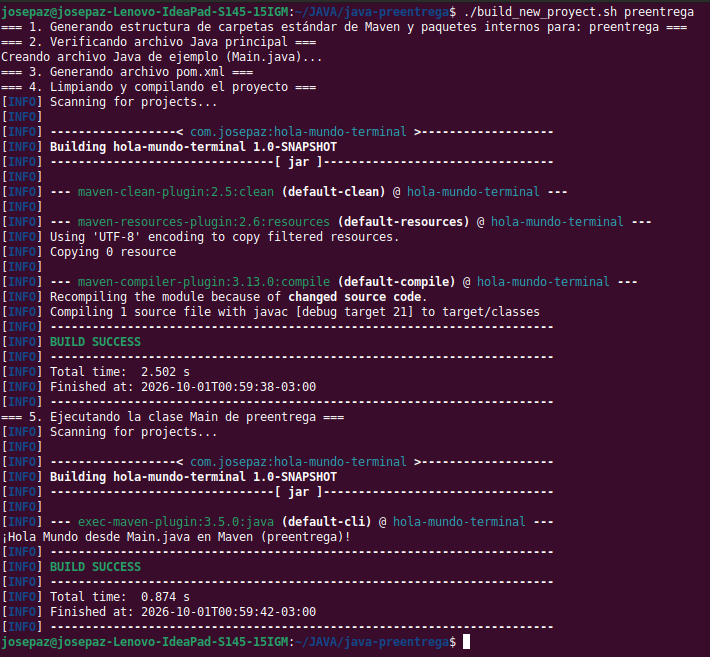
\includegraphics[width=0.9\textwidth]{construccion_nuevo_proyecto.png}
    \caption{Creación de un nuevo proyecto java}
    \label{fig:nuevo_proyecto_java}
\end{figure}


\subsection{Main.java}
\lstinputlisting[
    caption={Clase Main.java (Pre-entrega)}, 
    label={code:main_java}
]{./src/main/java/com/josepaz/preentrega/Main.java}

\subsection{Validador.java}
\lstinputlisting[
    caption={Clase Validador.java (Pre-entrega)}, 
    label={code:validador_java}
]{./src/main/java/com/josepaz/preentrega/util/Validador.java}

\subsection{Producto.java}
\lstinputlisting[
    caption={Clase Producto.java (Pre-entrega)}, 
    label={code:producto_java}
]{./src/main/java/com/josepaz/preentrega/model/Producto.java}

\subsection{ProductoService.java}
\lstinputlisting[
    caption={Clase ProductoService.java (Pre-entrega)}, 
    label={code:producto_service_java}
]{./src/main/java/com/josepaz/preentrega/service/ProductoService.java}


\subsection{ProductoNoEncontradoException.java}
\lstinputlisting[
    caption={Clase ProductoNoEncontradoException.java (Pre-entrega)}, 
    label={code:producto_no_encontrado_exception_java}
]{./src/main/java/com/josepaz/preentrega/exception/ProductoNoEncontradoException.java}

\subsection{StockInsuficienteException.java}
\lstinputlisting[
    caption={Clase StockInsuficienteException.java (Pre-entrega)}, 
    label={code:stock_insuficiente_exception_java}
]{./src/main/java/com/josepaz/preentrega/exception/StockInsuficienteException.java}


% ---------------------------------
% FIN DEL DOCUMENTO
% ---------------------------------
\end{document}

